\chapter{Evaluation}
\label{chapter|evaluation}

\section{Comparison of oro-server with other existing systems}
\label{sect|evaluation-oroserver}

\subsection{Performances Analysis}

\section{Experimental evaluation}
\label{sect|experimental-evaluation}

\subsection{Simulation of HRI interaction}
\label{sect|simulation}

\subsection{Case Studies}
\label{sect|casestudies}

This section reports on three small experiments conducted in the first half of
the PhD. Each of them illustrate one specific aspect of the knowledge base.

The first experiment, \emph{Point \& Learn} shows how the structure
(\emph{TBox}) of the knowledge base can be altered (in this case expanded) at
runtime through pointing interaction.

The second experiment, \emph{Odd One Out} shows how the knowledge model can be
used along with the categorization routines to isolate an ``odd" object, given
a simple context.

Lastly, the third case study is an implementation of the \emph{Spy Game} where
one of the player think of an object and the other one must guess by asking
questions.

It must be noted that these three experiments have been implemented on three
distinct robotic platforms: the \textit{BERT2} robot from the Bristol Robotics
Laboratory (a YARP-based architecture), the \textit{Rosie} robot from the
Technical University of Munich (a ROS-based architecture) and the \textit{Jido}
robot at LAAS-CNRS (based on the LAAS Pocolibs middleware).

\subsubsection{Knowledge acquisition: Point \& Learn}
\label{pointandlearn}

\begin{figure}
\centering

\centering
  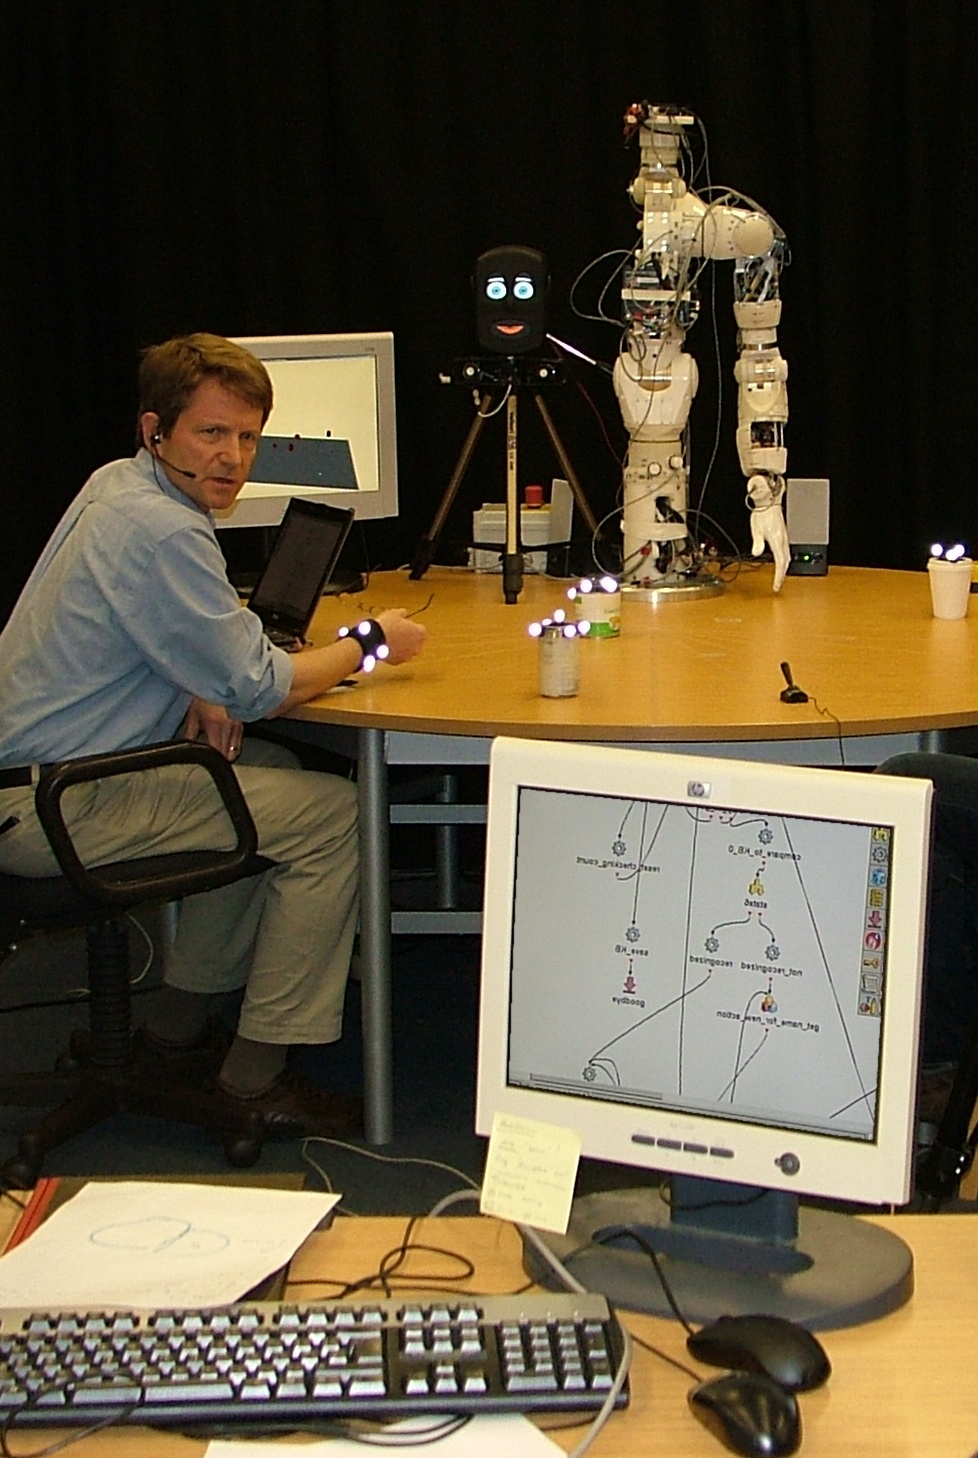
\includegraphics[width=0.4\columnwidth]{experiments/bristol_integration.jpg}
  \caption{Teaching the Bert robot new objects}
  \label{fig|bristol}

\end{figure}

We have implemented a \textit{Point \& learn} behaviour on the Bert robot~\cite{Lallee2010b} (Figure~\ref{fig|bristol}): the user shows an object to the robot, and if the robot sees it for the first time, it will ask for its name and type.

The object perception module relies on motion capture (VICON system) to identify and localize objects. A so-called \textit{primitive detection} module is responsible for updating ORO with the list of objects currently seen by the robot as well as their state (moving or not) and their relations to other objects (touching or not). On the other end, a human-robot interface based on the CLSU Toolkit\footnote{\url{http://cslu.cse.ogi.edu/toolkit/}} is in charge of speech recognition, speech synthesis and basic natural language processing.

By querying ORO for moving objects, the interface retrieves the object ID that has the focus of attention (last moving object), and asks the human for a name and a type if the object is new. Figure~\ref{tab|transcript_bert} reproduces a typical dialog with Bert.

At the end of this sequence, two more RDF statements are added to the robot knowledge base: \texttt{[5001 rdfs:label "coffee-cup"]} and \texttt{[5001 rdf:type Cup]}.

\begin{figure}[!ht]
\centering
	\begin{tabular}{r|p{0.6\columnwidth}}
	\chatN{bert} & Initializing... \textit{[about 5 sec]} ...What's next? \\
	\chatN{human} & \textit{[moves an object]} \\
	\chatN{bert} & \textit{[does not know the object]} How is it called? \\
	\chatN{human} & coffee-cup \\
	\chatN{bert} & Did you say coffee-cup? \\
	\chatN{human} & yes \\
	\chatN{bert} & Ok. Now I know. What kind of object is coffee-cup? \\
	\chatN{human} & a cup \\
	\chatN{bert} & Did you say cup? \\
	\chatN{human} & yes \\
	\chatN{bert} & So coffee cup is a cup. What's next? \\
	\end{tabular}
	\caption{Transcript of a chat with the Bert robot}
	\label{tab|transcript_bert}
\end{figure}

Due to the limitation of the speech recognition software, only a predefined set of names or types could be recognized, thus preventing the robot to add completely original objects.

\subsubsection{Odd One Out}
\label{odd_one_out}

\begin{figure}
\centering

    \subfigure[]{
        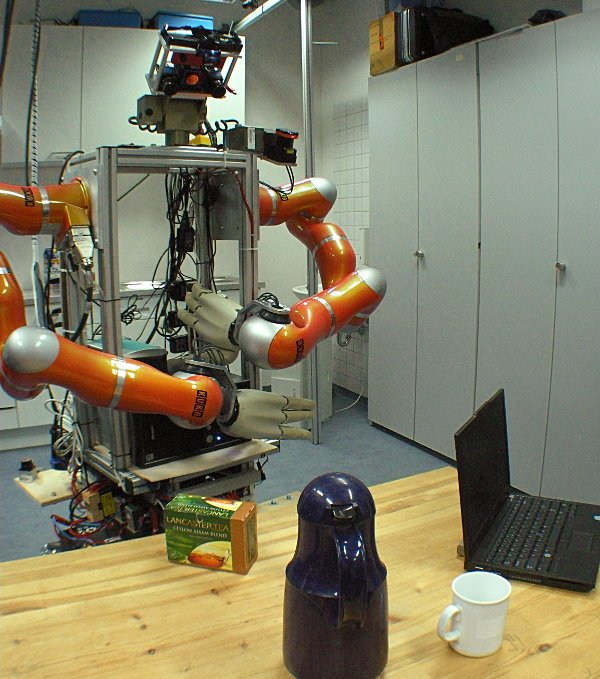
\includegraphics[width=0.4\textwidth]{experiments/kimp1.jpg}
    }
    \subfigure[]{
        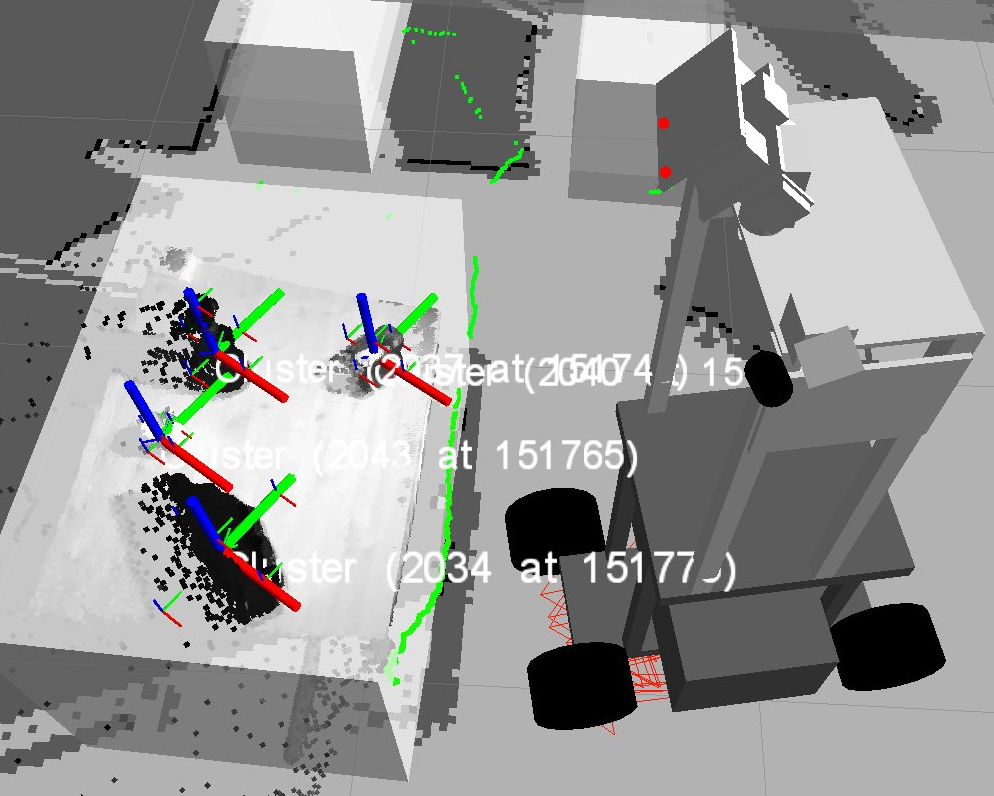
\includegraphics[width=0.4\textwidth]{experiments/rviz.png}
    }
\caption{(a) Rosie, looking for objects it may know, and (b) viewed in RViz. The clusters of point are given an unique identifier by the perception that allow the supervision create the link between the physical objects and their symbolic representation in ORO.}
\label{fig|kimpwatching}
\end{figure}


The \emph{Odd One Out} scenario extends the \textit{Point \& Learn} experiment and completes an on-going experiment at the IAS laboratory where a robot is asked to list missing items on a table being set, based on probabilistic reasoning on previously recorded observations.
%~\cite{Pangercic2009}.

We use ORO to introduce human interactions and common-sense reasoning: the robot picks an unknown object from the table, shows it to the user, and asks about its name and type (Figure~\ref{fig|kimpwatching}). The user continues to describe the object (through concepts) until a concept known by the robot is given. The learning process starts over again with another unknown object. Once all objects are learned, the robot tells which objects do not belong to a typical breakfast table (\textit{i.e.} objects that are neither food or tableware). The human interacts with the robot through a dedicated XMPP bridge, allowing to chat with the robot with a standard Jabber messaging client. Figure~\ref{tab|transcript_kimp} corresponds to a chat session with Rosie.

The supervision (\textsc{cram}\footnote{\textsc{cram} (Cognitive Robotic Abstract Machine) is a RPL-derived framework for rapid development of cognitive robot control programs we currently develop.}~\cite{Beetz2010}) automatically updates the ORO server whenever an object enters or leaves the field of view.
%(the perception is based on the \textsc{CoP} framework~\cite{Klank2009}). 
Therefore, the integration of ORO can be seen as an extension to
the robot's belief state that not only contains abstract identifiers
of the internal object representation used in plans, but also the
semantics and roles of objects in the scenario.

\begin{figure}[!ht]
\centering
	\begin{tabular}{r|p{0.7\columnwidth}}
	\chatN{rosie} & Servus! The Bavarian robot is up and fit! \\
	\chatN{rosie} & What is the name of the WHITE CLUSTER on the TABLE? \\
	\chatN{human} & "Rosie's mug" \emph{[Rosie adds \stmt{OBJ001 rdfs:label "Rosie's mug"} stmt]}\\
	\chatN{rosie} & What kind of object is Rosie's mug? \\
	\chatN{human} & Mug \\
	\chatN{rosie} & What is a Mug? \emph{[Rosie adds \stmt{OBJ001 rdf:type Mug} but it does not know the \emph{Mug} concept]}\\
	\chatN{human} & Tableware \emph{[Rosie knows about \emph{Tableware} - belongs to the common-sense ontology. It adds \stmt{Mug rdfs:subClassOf Tableware}]}\\
	 & (...) \\
	\chatN{rosie} &  What is the name of the BLACK CLUSTER on the TABLE? \\
	\chatN{human} & my laptop \\
	\chatN{rosie} & What kind of object is my laptop? \\
	\chatN{human} & Computer \\
	\chatN{rosie} & What is a Computer? \\
	\chatN{human} & Artifact \\
	\chatN{rosie} & Do you want me to learn more objects? \\
	\chatN{human} & no \\
	\chatN{rosie} & These objects are odd: my laptop \\
	\end{tabular}
	\caption{Transcript of a Jabber session with the robot Rosie. Compared to dialog with Bert (\ref{tab|transcript_bert}), we see here that the robot anchors the new objects in its already acquired knowledge.}
	\label{tab|transcript_kimp}
\end{figure}

By asking in loop the human for the categories of an object until it can connect it to a concept it already knows, the robot accurately anchors perception in its symbolic model and it is able to reason about it. At the end of the experiment, the robot identifies and returns the odd objects for the breakfast table (\textit{i.e.}, in our example, objects that are neither \texttt{Tableware} or \texttt{Food}).

An unexpected example of what the symbolic reasoning layer brings to more traditional robotic architectures emerged during the \emph{Odd One Out} experiment: the perception routines provided segmented blobs corresponding to objects, along with their colours. The supervision would then feed ORO with the visible objects. At some point, ORO suddenly refused to add an object. What seemed at first a communication bug between modules, was actually the consequence of a consistency check by ORO: Because of bad light conditions, the color recognition was not very reliable, and the same object was set to have two different colours at the same time. That was inferred as impossible by ORO and thus discarded. This kind of logical failure can be used to improve low-level perception results by ``closing the loop'' with high-level, symbolic knowledge.


\subsubsection{The Spy game}
\label{spygame}

This game is based on the traditional children game ``I Spy''. The idea is to discover the object or concept one of the participants is thinking of by asking questions such as: ``Is it green? Is it a machine? Is it on your left?'', etc. When playing, children exploit their knowledge about the world while categorizing and describing objects through useful discriminants that allow them to find out the answer as fast as possible while including perspective taking abilities~\cite{Moll2006}.

\begin{figure}
\centering

    \subfigure[]{
        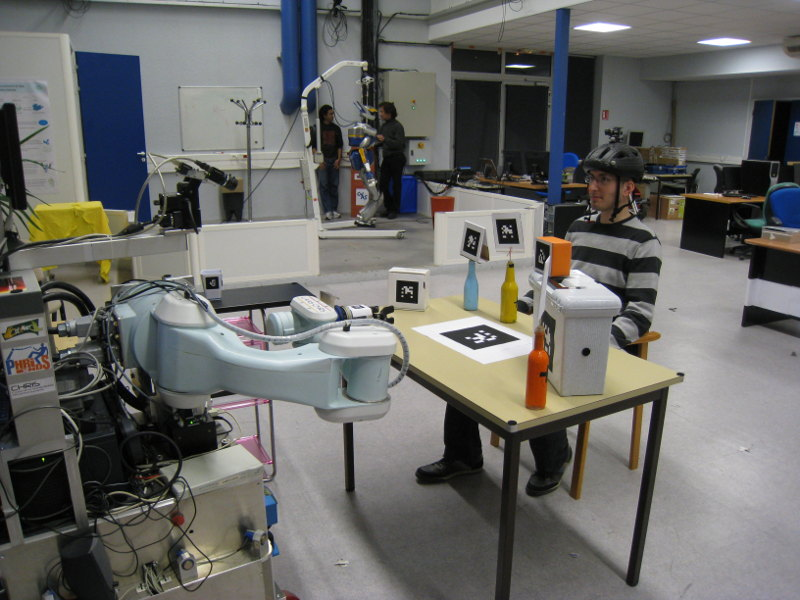
\includegraphics[width=0.4\textwidth]{experiments/spy-game-real.jpg}
    }
    \subfigure[]{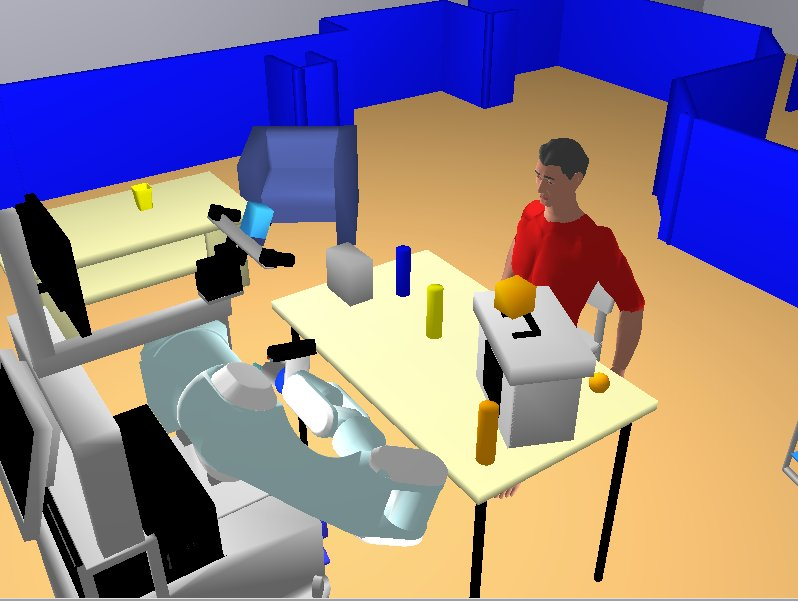
\includegraphics[width=0.4\textwidth]{experiments/spy-game-mhp.jpg}
    }
\caption{Spy game scenario: (a) Real environment and (b) 3D environment model, viewed in \textsc{Move3D}.}
\label{fig|spyGameScenario}
\end{figure}

The scenario for this game (Figure~\ref{fig|spyGameScenario}) consists on a face-to-face interaction where the human thinks of an object present in the environment, while the robot queries the human until either discovering the object or giving up, if no object was found. A categorization example is presented in Figure~\ref{fig|objectsSpyGame}. The game starts with the human user giving a first hint (communication is done through a keyboard and screen), allowing the robot to start the search filtering those objects that fulfill this first description. Based on this subset, ORO provides a descriptor (or set of descriptors) that allows a maximum discrimination among objects in the subset. The robot queries the user about the value of the descriptor (or the most discriminant among the set of descriptors) and with this new information, the current subset of objects is filtered again. The process is repeated until either obtaining a single object that fulfills all the descriptor values, or failing (\textit{i.e.} no object found). 

\begin{figure}[!h]
\centering
\begin{scriptsize}
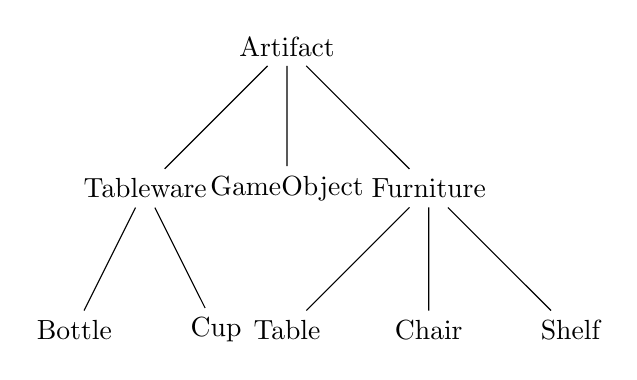
\begin{tikzpicture}[scale=1.2] %[level/.style={sibling distance=30mm/#1},scale=0.8]
	%[edge from parent fork down,
	%every node/.style={fill=black!30,rounded corners},
	%[parent anchor=east,child anchor=west,grow=east,
	%edge from parent/.style={thick,draw}]
	\node {Artifact}
	child {node {Tableware}
		child {node {Bottle}}
		child {node {Cup}}
		}
	child {node {GameObject}}
	child {node {Furniture}
			child {node {Table}}
			child {node {Chair}}
			child {node {Shelf}}};
\end{tikzpicture}
\end{scriptsize}
\caption{Example of object categorization used in the scenario.}
\label{fig|objectsSpyGame}			
\end{figure}

%Thing
%Object
%Tableware
%	- bottle: red, blue, yellow orange
%	- cup: white
%Furniture
%	- table: hrp2table, lowtable
%	- chair: chair1 and chair2
%	- shelf: pink_shelf
%GameObject: spacenavbox, orangebox, accesskit

We have integrated the game in the LAAS-CNRS Jido robot~\cite{Alami1998a}. Objects are identified through a tag-based vision approach\footnote{ARToolKit: \url{http://www.hitl.washington.edu/artoolkit/}} and motion capture is used for human tracking. Their descriptions regarding categories (type of object) and features (color, shape) are manually given in advance. Spatial relationships ({\tt front}, {\tt back}, {\tt left}, etc, and {\tt in}, {\tt on} and {\tt next to}) and visibility (only visible objects for both agents can be considered in the game) are automatically computed on-line by the \textsc{MHP/Move3D} geometric reasoner and planner~\cite{Marin2008}. Figure~\ref{fig|spyGameExample} shows an example of a round game.


\begin{figure}
\centering
	\begin{tabular}{r|p{0.7\columnwidth}}
		\chatN{human} & It is a tableware.\\
		\chatN{jido} & \emph{[retrieves possible objects: blue-bottle, yellow-bottle, orange-bottle, cup-with-handle]} \\
	 			& \emph{[keeps visible objects: blue-bottle, yellow-bottle, cup-with-handle]}\\
				& \emph{[obtains discriminants: type, color.]}\\
				& Which type of object is: bottle or cup? \\
		\chatN{human} & Bottle.\\
		\chatN{jido} & \emph{[obtains possible objects: blue-bottle, yellow-bottle.]}\\
				& \emph{[obtains discriminants: color.]}\\
				& What color the object is: blue or yellow?\\
		\chatN{human} & Blue.\\
		\chatN{jido} & \emph{[obtains possible objects: blue-bottle.]}\\
				& The object is the blue-bottle!	
	\end{tabular}\\
	\caption{Example of the robot playing Spy game.}
	\label{fig|spyGameExample}
\end{figure}

\subsection{First Interaction Experiment}
\label{sect|expe1}

In order to illustrate the approach presented in this paper, we have designed
the following daily life situation. Tom and Jerry are moving to London, so they
are packing things in boxes. The scenario takes places in the living-room,
where Jido (our robot) is observing while they move things here and there. To
assess the reasoning abilities of the robot they ask Jido for information
(entered through keyboard). Ideally, the robot should also perform actions when
required (e.g. hand an object when asking ``give me...''). However, since it is
out of the scope of this work, we do not include any motion from the robot's
side.

Perception of objects is done through a tag-based system and humans are
detected through motion capture. The robot knowledge base is pre-loaded with
the \emph{ORO Commonsense Ontology}\footnote{This ontology can be downloaded
from \url{http://oro.openrobots.org/}.}.  We next describe in detail two
situations where we can follow the internal robot's reasoning and the
interaction with the users.

\subsubsection{Implicit disambiguation through visual perspective taking}

Tom enters the room while carrying a big box (Figure~\ref{fig|vpt}, page 1). He
approaches the table and asks Jido to handle him the video tape: ``Jido, can
you give me the video tape''. The \textsc{Dialogs} module queries the ontology to
identify the object the human is referring to: \stmt{?obj \textbf{type} VideoTape}. 

There are two video tapes in the scene: one on the table, and another one
inside the cardboard box. Thus, the knowledge base returns both: $\Rightarrow$
\stmt{?obj = [videoTape1, videoTape2]}. 

However, only one is visible for Tom (the one on the
table). Thus, although there is an ambiguity from the robot's perspective
(since it can see both video tapes), based on the perspective of its human
partner it infers that Tom is referring to the video tape on the table, and not
the one inside the box which is not visible from his view. Therefore,
non-visible objects are removed obtaining: \stmt{?obj =[videoTape1]}.

Since only one object is available, the robot infers
that the human refers to it and would eventually execute the command, \ie give
it to the human. Alternatively, the robot could first verify with the human if
that was the object being referred to or not before proceeding to execute the
action. Table~\ref{table|ptbeliefs} lists the robot's beliefs about itself and
its human partner involved in this situation.

\begin{table}
\begin{center}
\begin{tabular}{l}
\hline
Robot's beliefs about itself (\emph{robot's model}):\\
\hline
  \hspace{0.7cm}\stmt{videoTape1 \textbf{type} VideoTape}\\
  \hspace{0.7cm}\stmt{videoTape1 \textbf{isOn} table}\\
  \hspace{0.7cm}\stmt{videoTape1 \textbf{isVisible} \textit{true}}\\
  \hspace{0.7cm}\stmt{videoTape2 \textbf{type} VideoTape}\\
  \hspace{0.7cm}\stmt{videoTape2 \textbf{isIn} cardBoardBox}\\
  \hspace{0.7cm}\stmt{videoTape2 \textbf{isVisible} \textit{true}}\\
\hline
\hline
Robot's beliefs about Tom (\emph{Tom's model}):\\
\hline
  \hspace{0.7cm}\stmt{videoTape1 \textbf{type} VideoTape}\\
  \hspace{0.7cm}\stmt{videoTape1 \textbf{isOn} table}\\
  \hspace{0.7cm}\stmt{videoTape1 \textbf{isVisible} \textit{true}}\\
  \hspace{0.7cm}\stmt{videoTape2 \textbf{type} VideoTape}\\
  \hspace{0.7cm}\stmt{videoTape2 \textbf{isIn} cardBoardBox}\\
  \hspace{0.7cm}\stmt{videoTape2 \textbf{isVisible} \textit{false}}\\
 \hline
\end{tabular}
\end{center}
\caption{Robot's beliefs about itself and its human partner.}
\label{table|ptbeliefs}
\end{table}

\subsubsection{Explicit disambiguation through verbal interaction and gestures}
\begin{figure}[!ht]
  \centering
  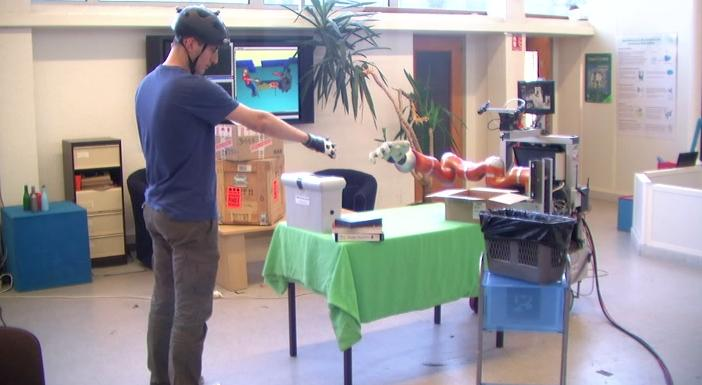
\includegraphics[width=0.9\linewidth]{images/dialogs/inTheBox2.jpg}
\caption{Jerry asks Jido for the content of the box by pointing at it.}
  \label{fig|pointing}
\end{figure}

In this situation, Jerry enters the
living room without knowing where Tom had placed the video tapes. So he first
asks Jido: ``What's in the box?''. Before the robot can answer the question it
has to figure out which box Jerry is talking about. Similar to the previous
situation, there are two available boxes: 

\begin{center}
\begin{tabular}{l}
\stmt{?obj \textbf{type} box}\\
\hspace{0.7cm}$\Rightarrow$ \stmt{?obj = [cardBoardBox, toolbox]}
\end{tabular}
\end{center}

However both are visible and the cognitive ambiguity resolution cannot be
applied. The only option is to ask Jerry which box he is referring to: ``Which
box, the toolbox or the cardboard box?'' Jerry could now simply answer the
question. Instead, he decides to point at it while indicating: ``This box''
(Figure~\ref{fig|pointing}). The robot's perception identifies the {\tt
cardBoardBox} as being pointed at and looked at by the human and updates the
ontology with this new information using a rule available in the commonsense
ontology ({\tt \textbf{pointsAt}(?ag, ?obj) $\land$ \textbf{looksAt}(?ag, ?obj) $\to$
\textbf{focusesOn}(?ag, ?obj)}) The \textsc{Dialogs} module is then able to merge both
sources of information, verbal (``this'') and gestural to distinguish the box
Jerry refers to.

\begin{center}
\begin{tabular}{l}
\stmt{Jerry \textbf{pointsAt} carboardBox}\\
\stmt{Jerry \textbf{looksAt} carboardBox}\\
$\to$ \stmt{Jerry \textbf{focusesAt} carboardBox}\\
\hspace{0.7cm}$\Rightarrow$ \stmt{?obj = [cardBoardBox]}
\end{tabular}
\end{center}

Finally, the \textsc{Dialogs} queries the ontology about the content of the box
and the question can be answered: ``Jido-E''. Note that the object's label is
used instead of its ID. This way we enhance interaction using familiar names
given by the users.

\begin{center}
\begin{tabular}{l}
\stmt{?obj \textbf{isIn} cardBoardBox}\\
\hspace{0.7cm}$\Rightarrow$ \stmt{?obj = videoTape2}\\
\end{tabular}
\end{center}

At this point Jerry wants to know where the other tape is, and that is exactly
what he asks Jido: ``And where is the other tape?''. In this occasion, the
\textsc{Dialogs} module is able to interpret that Jerry is not referring to the
video which they were just talking about, but to the other one:

\begin{center}
\begin{tabular}{l}
\stmt{?obj \textbf{type} VideoTape}\\
\stmt{?obj \textbf{differentFrom} videoTape2}\\
\hspace{0.7cm}$\Rightarrow$ \stmt{?obj = [videoTape1]}
\end{tabular}
\end{center}

Since there is only one possible ``other'' video (there are only two videos in
the scene), it can directly answer Jerry: ``The other tape is on the table and
next to the toolbox.''

\begin{center}
\begin{tabular}{l}
\stmt{videoTape1 \textbf{isOn} table}\\
\stmt{videoTape1 \textbf{isNextTo} toolbox}
\end{tabular}
\end{center}


\subsection{Second Interaction Experiement}
\label{sect|expe2}

\begin{figure}
    \centering
    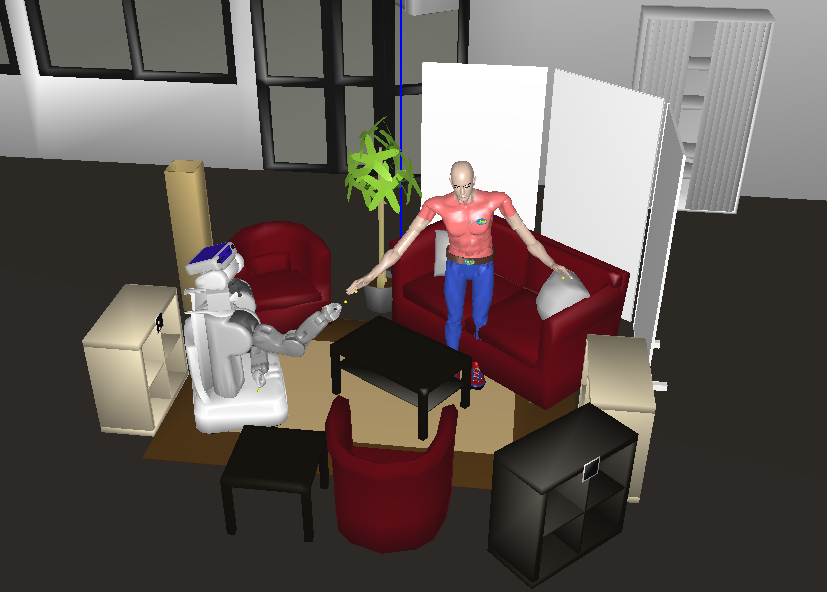
\includegraphics[width=0.7\columnwidth]{experiments/adream-livingroom.png}
    \caption{The ``Living room'' setup}
    \label{fig|livingroom}
\end{figure}


